%%%%%%%%%%%%%%%%%%%%%%%%%%%%%%%%%%%%%%%%%%%%%%%%%%%%%%%%%%%%%%%%%
%_____________ ___    _____  __      __ 
%\____    /   |   \  /  _  \/  \    /  \  Institute of Applied
%  /     /    ~    \/  /_\  \   \/\/   /  Psychology
% /     /\    Y    /    |    \        /   Zürcher Hochschule 
%/_______ \___|_  /\____|__  /\__/\  /    fuer Angewandte Wissen.
%        \/     \/         \/      \/                           
%%%%%%%%%%%%%%%%%%%%%%%%%%%%%%%%%%%%%%%%%%%%%%%%%%%%%%%%%%%%%%%%%
%
% Project     : Latex Vorlage SemArbeit
% Title       : 
% File        : dispositionBachelorarbeit.tex Rev. 00
% Date        : 11.2013
% Author      : Till J. Ernst
%
%%%%%%%%%%%%%%%%%%%%%%%%%%%%%%%%%%%%%%%%%%%%%%%%%%%%%%%%%%%%%%%%%
\chapter*{Disposition Bachelorarbeit}\label{chap.dispo}
\glsresetall
% Kapitel Ausgangslage
\begin{tabularx}{17cm}{lX}
Name des Schreibenden & Till Ernst \\
Name des Referenten & Prof. Dr. phil. habil. Daniel Süss \\
Titel der Arbeit & Hat Multitasking einen Einfluss auf das eigene Glück? Auswirkung von Medien-Multitasking auf das subjektive Wohlbefinden von Studenten\\
\end{tabularx}
% Fragestellung -------------------------------------------------
\section*{Fragestellung / Annahme}\label{section.fragestellung}
\textbf{Hauptfragestellung:} Beeinflusst die Häufigkeit und die Fähigkeit bezogen auf Medien-Multitasking das subjektive Wohlbefinden von Studenten? 
\par
\textbf{Nebenfragestellung:} Wenden Studenten, die mehrere Rollen neben dem Studium ausüben, aufgrund ihrer Rollenvielfalt ein höheres Mass an Medien-Multitasking an, bezogen auf die restlichen Studenten? \par
\textbf{Annahme:} Die Häufigkeit und die Fähigkeit wie Medien-Multitasking angewendet wird, wirkt sich auf das subjektive Wohlbefinden von Studierenden aus.
Gemäss aktuellen Studien \cite<e.g.,>{Sanbonmatsu2013, Rosen2013} wird davon ausgegangen, dass Multitasking unter anderem von der Fähigkeit, Ablenkung abzublocken, Überschätzen der eigenen Fähigkeit, Impulsivität, Sensation Seeking oder starker Belohnungs- und Nutzenorientierung abhängig ist. Bisher konnte der direkte Zusammenhang zwischen Medien-Multitasking und Wohlbefinden nicht nachgewiesen werden \cite{Shih2013}. \\
Diese Studie geht davon aus, dass der Einfluss von einem in hohem Mass angewendeten Medien-Multitasking, mit gleichzeitiger Überschätzung der eigenen Fähigkeit, mit einem geringeren subjektiven Wohlbefinden einhergeht.\\
Zudem wird angenommen, dass Studierende mit mehreren Rollen, die sie neben dem eigentlichen Studium erledigen (z.B.: Familie, Erwerb, etc.), mehr Medien-Multitasking anwenden. Dies könnte unter Umständen daran liegen, da sie sich durch das Multitasking eine Zeitersparnis erhoffen (Bewältigungsstrategie).\\ 
Der Trend von Medien-Multitasking ist stetig am steigen, was unter anderem auf die rasante Entwicklung von neuen Medien und einer sich stetig entwickelnden Technologie zurückzuführen ist \cite{Lee2012}. Aus diesem Grund soll sich die Studienpopulation aus Studierenden aus Universitäten und Fachhochschulen zusammensetzen, da diese sozusagen an vorderster Front in einem direkten Austausch mit diesen Technologien und Medien stehen. 
% Hypothese -----------------------------------------------------
\section*{Hypothese}\label{section.hypothesen}
\textbf{Haupthypothesen:}
\begin{itemize}
    \item Studierende, die am häufigsten Medien-Multitasking anwenden sind diejenigen, die am wenigsten Fähig sind Ablenkung abzublocken und somit Medien-Multitasking zu praktizieren. Dies wiederum wirkt sich negativ auf das subjektive Wohlbefinden dieser Studenten aus. 
     \item Studierende mit einer hohen Rollenvielfalt wenden vermehrt Medien-Multitasking an, um damit Rollenkonflikte zu lösen, die durch Zeitnot entstanden sind.
\end{itemize}
\textbf{Arbeitshypothesen:}
\begin{itemize}
    \item Zwischen der Häufigkeit wie Medien-Multitasking angewendet wird und dem subjektiven Wohlbefinden besteht ein negativer Zusammenhang. Je mehr Media-Multitasking angewendet wird, desto negativer wirkt sich dies auf das subjektive Wohlbefinden aus.
    \item Zwischen der Fähigkeit Medien-Multitasking zu betreiben und dem subjektiven Wohlbefinden besteht ein positiver Zusammenhang. Fähige Studenten können besser zwischen schädlichem und nützlichen Medien-Multitasking unterscheiden und beeinflussen dadurch das eigene subjektive Wohlbefinden positiv.
    \item Zwischen der Fähigkeit von Studierenden Medien-Multitasking zu betreiben und der Häufigkeit besteht ein negativer Zusammenhang. Je fähiger Studierende im Umgang Medien-Multitasking sind, desto weniger werden sie Medien-Multitasking anwenden.
\end{itemize}
\section*{Art der Arbeit}\label{section.artArbeit}
Bei dieser Arbeit handelt es sich um eine empirische Bachelorarbeit mit quantitativem Charakter. 
% Theoretischer Hintergrund --------------------------------------
\section*{Theoretischer Hintergrund / Stand der Forschung}\label{section.forschung}
In einer Zeit, in der neue Medien wie Pilze aus dem Boden schiessen, ist das Medien-Medien-Multitasking (MMM) - das Konsumieren von mehr als einem Medienelement oder Medienstrom zur gleichen Zeit (z.B.: Mobile, Mail, iPod) - ein Phänomen, das vor allem bei jungen Leuten stark zunimmt \cite{Rideout2010}. Einer der Hauptgründe für die rasante Zunahme des Medien-Multitasking wird dem Computer zugeschrieben, der durch die immer wiederkehrenden Arbeitsunterbrechungen (z.B.: Download von Files, Installation von Software, etc.) und sporadischen Meldungen an den Benutzer (z.B.: Benachrichtigung eingehender Mails, Informationen über den Betriebszustand, etc.) richtiggehend zum Multitasking animiert \cite{Foehr2006}.  Untersuchungen haben gezeigt, dass ein exzessives Medien-Multitasking mit einer erhöhten Risikofreude und einer Sensationslüsternheit (engl. sensation-seeking) einhergeht \cite{Foehr2006}. Aus einer weiteren Studie geht hervor, dass je mehr eine Person zu Multitasking neigte, desto höher scheint dies mit einem klinischen Symptom wie Depression, Manie, Narzissmus, antisozialer Persönlichkeitsstörung und Paranoia einher zu gehen \cite{Rosen2013}. Die Art und weise wie Multitasking eingesetzt wird, dient als weiterer Faktor für die Unterscheidung von extern auferlegten (z.B.: im Job) und einem selbst auferlegten (z.B.: in der Freizeit) Multitasking \cite{Shih2013}. \\
Viele dieser uns alltäglichen, mental anspruchsvollen Multitasking-Handlungen beziehen das Arbeitsgedächtnis mit ein. Daraus lässt sich schliessen, dass die Beschränkung des Arbeitsgedächtnis mit der Beschränkung des Multitaskingvermögens einhergehen könnte. Dies wiederum könnte sich auf die Kapazitätsgrenze der sich überlappenden Stirn- und Scheitellappen zurückführen lassen \cite{Klingberg2008}. Der aktuelle Stand der Forschung ist sich uneins, ob es möglich ist das Arbeitsgedächtnis zu schulen und dadurch das Medien-Multitasking zu verbessern. Gewisse Studien deuten darauf hin, dass sich mittels Training das Arbeitsgedächtnis verbessert \cite{Hernstein1986, Feuerstein1985, Stankov1986}. Würde sich dadurch der sogenannte \textquotedblleft Flynn-Effekt\textquotedblright \ bestätigen \cite{Flynn1987}, der auf positive Veränderungen des Arbeitsgedächtnis zurückzuführen ist, könnte man davon ausgehen, dass der Umgang mit den Medien zu einer Verbesserung des Arbeitsgedächtnisses und der damit einhergehenden Problemlösekompetenz in der Bevölkerung führen würde \cite{Klingberg2008}. Einige Studien weisen hindessen darauf hin, dass Personen, die Multitasking anwenden, signifikant schlechter abschneiden als die Nicht-Multitasker \cite{Spitzer2012}.\\
Subjektives Wohlbefinden und Wohlbefinden wird in der Literatur sehr unterschiedlich verwendet. In dieser Arbeit wird jedoch das Wohlbefinden als ein Konstrukt der positiven Psychologie verstanden \cite{Carr2011}. Die Positive Psychologie hat einen wissenschaftlichen und eine klinischen Anspruch \citeyear<ebda.,>{Carr2011}. Die wissenschaftliche Auseinandersetzung innerhalb der Positiven Psychologie befasst sich mit dem Verstehen und dem Verbessern von positiven Aspekten im Leben (z.B.: Glück und Wohlbefinden, positive menschliche Eigenschaften, Entwicklung von positiven Beziehungen, etc.) \cite{Seligman2004}. Die Messung des subjektiven Wohlbefindens geht auf Studien des Professors Ed Diener \citeyear{Myers:1995} zurück. Seither wurden diverse Konstrukte zur Messung des subjektiven Wohlbefinden entwickelt, die vom einfachen Fragebogen \cite{Carr2011}, zu einer 2-Item-Skala \cite{Fordyce:1988}, dem \textquotedblleft Oxford Happiness Questionnaire\textquotedblright \ \cite{Hills2002} oder der Zeitpunkt-Messung von \citeA{Hektner:2007} reichen.\\
In dieser Studie soll angeschaut werden, ob sich das Multitasking, vor allem das Medien-Multitasking, auf das subjektive Wohlbefinden auswirkt. Dazu soll aufgrund der Theorie im Vorfeld versucht werden Anhaltspunkte zu finden, die für eine mögliche Auswirkung auf das subjektive Wohlbefinden hin deuten.
% Methode --------------------------------------------------------
\section*{Methode (Studiendesign)}\label{section.methode}
Bei dieser Bachelorarbeit handelt es sich um eine Querschnitts-Studie, in der mittels Fragebogen in erster Linie das subjektive Wohlbefinden, die Häufigkeit von angewendetem Medien-Multitasking und die Fähigkeit, wie Medien-Multitasking betrieben wird, empirisch erhoben werden soll. Die erhobenen Daten sollen mittels deskriptiver Statistik ausgewertet werden.
\subsection*{Untersuchungsplan und Vorgehen}

\begin{figure}[H]
	\centering
	    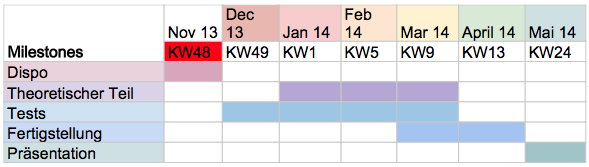
\includegraphics[width=0.9\textwidth]
		{images/Untersuchungsplan_Grob.png}
	\caption{Untersuchungsplan grob - Bachelorarbeit}
	\label{fig.UntersuchungsplanGrob}
\end{figure}
Der Untersuchungsplan unterteilt sich grob in fünf Kategorien (Milestones): Disposition, theoretischer Teil, Tests, Fertigstellung und Präsentation (ein detaillierter Untersuchungsplan ist im Anhang zu finden).\par
\textbf{Disposition:} Die Kategorie Disposition beinhaltet den Untersuchungsplan, die Korrektur der Disposition und die Abgabe am 29.11.2013.\par
\textbf{Theoretischer Teil:} Der theoretische Teil umfasst im groben die gesamte theoretische Aufarbeitung der Bachelorarbeit. Unterteilt wird dieser Teil in Einleitung, Multitasking, subjektives Wohlbefinden, Theorie zu den Tests, Diskussion und Fertigstellung der Arbeit. \par
\textbf{Tests:} Die Kategorie Tests beinhaltet das Einlesen in die Tests, das Schreiben des Theorieteils über die verwendeten Tests, die Koordination und das Einarbeiten mit den Testwerkzeugen (z.B.: Unipark, Surveymonkey, etc.), das Zusammenstellen der Umfrage, das Verfassen des Mailings für die Probandengewinnung und Sammeln der Kontaktadressen (Unis, Fachhochschulen), das Versenden und Durchführen der Umfrage per Mail (inkl. Abwarten und gegebenenfalls wiederholen), die Einarbeitung mit dem freien Statistik-Tool R \cite{Luhmann2013}, das Auswerten der Resultate mit R, die Aufbereitung der Ergebnisse und das dokumentieren der Ergebnisse.\par
\textbf{Fertigstellung:} In der Fertigstellung wird Zeit für eine allfällige Überarbeitung der Arbeit eingeplant, die externe Durchsicht und Korrektur, die eigene Korrektur, das Binden der Arbeit und die Abgabe in Kalenderwoche 22.\par
\textbf{Präsentation:} Die Präsentation besteht aus dem Erarbeiten eines wissenschaftlichen Posters und der Präsentation des Posters in KW25.\par
\subsection*{Datenerhebung}
Im Fokus dieser Untersuchung steht die Erfassung, wie häufig Medien-Multitasking praktiziert wird, wie fähig diese Probanden sind, Medien-Multitasking auszuführen und wie hoch ihr subjektives Wohlbefinden dabei ist. \\ 
Des Weiteren werden demographische Daten wie Alter, Geschlecht, Nationalität, Studienrichtung, bereits absolvierte Ausbildung, Beruf neben dem Studium und Familienstand abgefragt.\\
Die Erfassung dieser Daten erfolgt mittels Fragebogen, der aus einzelnen Fragebögen, oder Teilen davon, zusammengesetzt ist. Folgende Fragebögen werden für diese Untersuchung verwendet:
\begin{enumerate}
    \item \textit{Media Use Questionnaire} für die Häufigkeit von angewendetem Medien-Multitasking \cite{Ophir2009}.
    \item \textit{Operation Span Task - OSPAN} für die Messung der Fähigkeit für Medien-Multitasking mittels Kapazität des Arbeitsgedächtnisses \cite{Unsworth2005, Sanbonmatsu2013}.
    \item \textit{FLZ - Fragen zur Lebenszufriedenheit} für die Erfassung des subjektiven Wohlbefindens \cite{Braehler1999}.
\end{enumerate}
\subsection*{Stichprobe und Rekrutierung}
Die Stichprobengrösse ist für die Untersuchung der Nebenfragestellung relevant, da hier ein Signifikanzniveau angestrebt wird. Für die Beantwortung der Hauptfragestellung ist die Stichprobengrösse von untergeordneter Rolle, da dies mit einer Korrelation durchgeführt wird. Grundsätzlich kann hier gesagt werden, das je mehr Probanden gefunden werden desto besser ist dies für die Auswertung.\par
Anhand der Nebenfragestellung wird eine Stichprobengrösse von insgesamt 176 Personen angestrebt (88 Personen mit multiplen Rollen und 88 Personen mit einer einzigen Rolle). Diese Stichprobengrösse wurde mittels G*Power für einen t-Test für unabhägige Stichproben mit einem mittleren Effekt von $d = 0.5$, einem Signifikanzniveau von $\alpha=0.05$ und einer Teststärke von $1-\beta=0.95$ berechnet.
Die Rekrutierung der Studierenden erfolgt mittels Mailing in den deutschsprachigen Fachhochschulen und Universitäten.\par
\textbf{Einschlusskriterien:}
Studenten von Universitäten und Fachhochschulen mit keiner oder mehreren Rollen neben dem Studium. Als eine Rolle werden Tätigkeiten oder Verpflichtungen angeschaut, die zusammen gleich einem Drittel oder mehr des Pensum des Studiums entsprechen (z.B.: die zusätzliche Rolle oder Rollen sollen vom Aufwand pro Woche mindestens einem Drittel der durchschnittlichen Anzahl Stunden Studium pro Woche entsprechen).\par
\textbf{Ausschlusskrieterien:}
Ausgeschlossen werden Studierende eines Fernstudiums, da hier weitere Bedingungen gegeben sind, die eine Vergleichbarkeit erschwert.
Es werden nur Personen berücksichtigt, die der deutschen Sprache mächtig sind. Der Fragebogen wird lediglich auf Deutsch zur Verfügung gestellt.
\subsection*{Statistik}
Der Zusammenhang zwischen den einzelnen Variablen \textquotedblleft Häufigkeit\textquotedblright \ von angewendetem Medien-Multitasking, \textquotedblleft Fähigkeit\textquotedblright, Ablenkung abzublocken und dem \textquotedblleft subjektiven Wohlbefinden\textquotedblright, wird mittels Korrelation berechnet. Dabei soll ein mittlerer Zusammenhang mittels Produkt-Moment-Korrelationskoeffizienten (Pearson-Korrelations-Koeffizienten $|r|=0.3$) zwischen den einzelnen Variablen nachgewiesen werden. Um den Zusammenhang der Haupthypothese zu berechnen wird eine Partialkerrelation zwischen den Variablen Häufigkeit, Fähigkeit und subjektivem Wohlbefinden gebildet.\\
Für die Medien-Multitasking Häufigkeit soll der \textit{Medien Multitasking Index - MMI} aus dem \textit{Media Use Questionnaire} gebildet werden \cite{Ophir2009}.\par
Für die Signifikanzprüfung der unterschiedlichen Rollen soll mittels t-Test untersucht werden, ob sich die Mittelwerte der Studenten mit mehreren Rollen gegenüber den Studenten mit nur einer Rolle systematisch (signifikant) voneinander unterscheiden. Es wir ein mittlerer Effekt ($d=0.5$) erwartet. Das Signifikanzniveau wir auf ($\alpha=0.05$) angesetzt und die Teststärke mit ($1-\beta=0.95$) angewendet.\\
Die Hypothese geht davon aus, dass Studierende mit mehreren Rollen einem höheren Medien-Multitasking ausgesetzt sind als Studierende mit nur einer Rolle. Daraus ergibt sich eine gerichtete Hypothese, die gegen die Nullhypothese getestet werden soll.\par
Neben der Häufigkeit wird das subjektive Wohlbefinden analog dazu mit einem gerichteten t-Test untersucht.
% Abgrenzung -----------------------------------------------------
\section*{Abgrenzung}\label{section.abgrenzung}
In dieser Arbeit soll das subjektivem Wohlbefinden als Konstrukt im Zusammenhang mit der Positiven Psychologie behandelt werden. Eine weitere allgemeine Abhandlung und die Entstehungsgeschichte soll aus Redundanzgründen mit der bereits erstellten Seminararbeit \cite{Ernst2013} wo immer möglich vermieden werden.
%\section*{}\label{section.}